% \documentclass[linenumbers,floatfix,ApJL,twocolumn]{aastex631}
\documentclass[floatfix,ApJL,twocolumn]{aastex631}

\usepackage{amssymb}
\usepackage{amsmath}
\usepackage{microtype}
\usepackage{url}
\usepackage{xspace}
\usepackage{xcolor}
\usepackage{ifxetex}
\ifxetex
\usepackage{fontspec}
\defaultfontfeatures{Extension = .otf}
\fi
\usepackage{fontawesome5}

\setlength{\parindent}{3.0ex}


% Projects:
\newcommand{\project}[1]{\textsf{#1}}

\newcommand{\python}{\project{Python}}
\newcommand{\cython}{\project{Cython}}
\newcommand{\cpp}{\project{C++}}
\newcommand{\jupyter}{\project{Jupyter}}

\newcommand{\exoplanet}{\project{exoplanet}}
\newcommand{\lightkurve}{\project{lightkurve}}
\newcommand{\starry}{\project{starry}}
\newcommand{\theano}{\project{Theano}}
\newcommand{\pymc}{\project{PyMC3}}
\newcommand{\celerite}{\project{celerite}}
\newcommand{\dynesty}{\project{dynesty}}
\newcommand{\astroquery}{\project{astroquery}}
\newcommand{\scipy}{\project{scipy}}
\newcommand{\jupytext}{\project{jupytext}}
\newcommand{\sphinx}{\project{sphinx}}
\newcommand{\jupyterbook}{\project{Jupyter-book}}
\newcommand{\arviz}{\project{ArviZ}}
\newcommand{\nbconvert}{\project{nbconvert}}


\newcommand{\tess}{\project{TESS}}
\newcommand{\kepler}{\project{Kepler}}
\newcommand{\gaia}{\project{Gaia}}

\newcommand{\mast}{\project{MAST}}
\newcommand{\exofop}{\project{ExoFOP}}

\newcommand{\tessAtlas}{\project{TESS Atlas}}

% math
\newcommand{\T}{\ensuremath{\mathrm{T}}}
\newcommand{\dd}{\ensuremath{ \mathrm{d}}}
\newcommand{\unit}[1]{{\ensuremath{ \mathrm{#1}}}}
\newcommand{\bvec}[1]{{\ensuremath{\boldsymbol{#1}}}}


\DeclareMathOperator{\invG}{Inv-\mathnormal{\Gamma}}
\DeclareMathOperator{\N}{\mathcal{N}}
\DeclareMathOperator{\U}{\mathcal{U}}
\DeclareMathOperator{\Un}{\mathcal{U}}
\DeclareMathOperator{\Par}{\mathcal{P}ar}
\DeclareMathOperator{\tmin}{\mathnormal{t_{\rm min}}}
\DeclareMathOperator{\tmax}{\mathnormal{t_{\rm max}}}





%% affiliation shortcuts
\newcommand{\SPA}{School of Physics and Astronomy, Monash University, Clayton VIC 3800, Australia}
\newcommand{\OzGravMonash}{OzGrav: The ARC Centre of Excellence for Gravitational Wave Discovery, Clayton VIC 3800, Australia}
\newcommand{\AMNH}{Department of Astrophysics, American Museum of Natural History, New York, NY 10024, USA}
\newcommand{\CCA}{Center for Computational Astrophysics, Flatiron Institute, New York, NY 10010, USA}
\newcommand{\CUNY}{Graduate Center, City University of New York, 365 5th Avenue, New York, NY 10016, USA}
\newcommand{\BMCC}{Department of Science, BMCC, City University of New York, New York, NY 10007, USA}








\newcommand{\atlasUrl}{\href{http://catalog.tess-atlas.cloud.edu.au/}{catalog.tess-atlas.cloud.edu.au}}


\newcommand{\toiTemplateLink}{\href{https://github.com/dfm/tess-atlas/blob/main/src/tess_atlas/notebook_templates/toi_template.py}{github.com/dfm/tess-atlas/.../toi\_template.py}}

\newcommand{\paperPlotsLink}{\github{https://github.com/dfm/tess-atlas/blob/main/paper/figures/make_plots.py}}
\newcommand{\exoplanetOptimization}{\github{https://github.com/exoplanet-dev/pymc3-ext##optimization}}
\newcommand{\exoplanetDocs}{\href{https://docs.exoplanet.codes}{https://docs.exoplanet.codes/}}





%% Confirmed Numbers
% https://exoplanetarchive.ipac.caltech.edu/docs/counts_detail.html
% https://exoplanetarchive.ipac.caltech.edu/index.html
\newcommand{\numConfirmedPlanets}{5,090} % 
\newcommand{\numCandidatesRemaining}{6,959}
\newcommand{\numTessCandidates}{5,488} % 
\newcommand{\numTessPlanets}{227}


%% Atlas numbers
\newcommand{\numAnalysed}{2,833}
\newcommand{\failPercent}{3\%}
\newcommand{\numAnalysedMulti}{357}
\newcommand{\numMultiSystems}{157}
\newcommand{\numAnalysedSingle}{81}
\newcommand{\cpuHrs}{$\sim80,000\ \rm{Hrs}$}

\newcommand{\red}{\textcolor{red}}


\newcommand{\textuit}[1]{\textit{\underline{#1}}}



%% Numbers
% https://exoplanetarchive.ipac.caltech.edu/docs/counts_detail.html
% https://exoplanetarchive.ipac.caltech.edu/index.html


\newcommand{\numConfirmedPlanets}{5,090} % 
\newcommand{\numCandidatesRemaining}{6,959}

\newcommand{\numTessCandidates}{5,488} % 
\newcommand{\numTessPlanets}{227}
\newcommand{\numAnalysed}{2,833}
\newcommand{\numAnalysedMulti}{151}
\newcommand{\numAnalysedSingle}{68}
\newcommand{\cpuHrs}{$\sim80,000\ \rm{Hrs}$}

%% links
\newcommand{\atlasUrl}{\url{http://catalog.tess-atlas.cloud.edu.au/}}





\shorttitle{The \tess\ Atlas}


\begin{document}

\title{The \tessAtlas: an open-source living catalog of TESS transit fits}

\correspondingauthor{Daniel Foreman-Mackey}
\email{foreman.mackey@gmail.com}

\author[0000-0002-4146-1132{Avi Vajpeyi}
\affiliation{
    School of Physics and Astronomy,
    Monash University,
    Clayton VIC 3800,
    Australia
}
\affiliation{
OzGrav: The ARC Centre of Excellence for Gravitational Wave Discovery,
Clayton VIC 3800,
Australia
}

\author[0000-0002-9328-5652]{Daniel Foreman-Mackey}
\affiliation{
    Center for Computational Astrophysics,
    Flatiron Institute,
    162 5th Ave,
    New York, NY 10010
}







\begin{abstract}
We present the \tess\ Atlas, a living catalog of candidate exoplanet parameter estimates, from two-minute cadence \tess\ data from \red{2018-2021}.
This catalog contains posterior estimates for \red{\numAnalysed} \tess\ Objects of Interest, including \red{\numMultiSystems} multi-planet candidate systems and \red{\numAnalysedSingle} candidates having data for a single transit.
Our analysis utilises the No-U-Turns Markov chain Monte Carlo algorithm to sample the parameter space with a circular transit model implemented in \exoplanet.
We provide software, \jupyter\ notebooks and output files for all analyses so they can be easily reproduced, modified, and utilised in the future.
\end{abstract}

% info on sectors: https://heasarc.gsfc.nasa.gov/docs/tess/sector.html

\keywords{%
  methods: data analysis ---
  methods: statistical ---
  miscellaneous --- catalogs --- surveys
}


\section{Introduction} \label{sec:intro}

In March 2022, NASA's exoplanet archive~\citep{Akeson:2013:PASP} surpassed five thousand confirmed exoplanets, a milestone made possible by data from several observatories, including the Transiting Exoplanet Survey Satellite TESS~\citep{Ricker:2015:JATIS, Stassun:2018:AJ, Stassun:2019:AJ, Guerrero:2021:ApJS}.
The confirmed exoplanets exhibit a wide range of masses, compositions, and radii.
Some of these planets are also located within their planetary systems' habitable zone, e.g. TRAPPIST-1defg~\citep{Gillon:2017:Natur, Wolf:2017:ApJL, Agol:2021:PSJ}, Teegarden's Star bc~\citep{Zechmeister:2019:AA}, etc.
Furthermore, the population of these exoplanets has fuelled research into planetary system architecture, planetary formation and evolution, and updated exoplanet occurrence rates~\citep{Winn:2015:ARAA, Sing:2016:Natur, Emsenhuber:2021:AA, Zhu:2021:ARAA}.
These analyses will be more informative with a bigger sample of exoplanets and more precise estimates of the planet's characteristics.
This list of $\sim5,000$ exoplanets may be dramatically increased once the $\sim6,000$ candidates awaiting validation are processed, more than half of which are \tess\ Objects of Interest (TOIs).

\avi{Hmm this is lacking a clear discussion on motivation}
In this paper, we re-measure the planet parameters for all \red{\numAnalysed} of the TOIs with two-minute cadence observations from \red{2018 through 2021}, assuming that the TOIs are from transiting planets.
Our analysis provides realistic uncertainty estimates for the TOI's best-fit parameters and a uniform database of transiting exoplanet posterior estimates, which may be leveraged for future follow-up studies.
Additionally, we build and publicly distribute \jupyter\ notebooks for the end-to-end analysis of each TOI, making the data products easy to reproduce and access.
The notebooks are available on the catalog website (\atlasUrl).

The remainder of the paper is organised as follows.
Section~\ref{sec:method} outlines the procedures to analyse each TOI and generate the \tessAtlas.
The catalog results are summarised in Section~\ref{sec:results}.
The catalog data products, and software to reproduce the results available online as supplementary materials (\atlasUrl).
Finally, we discuss caveats and provide concluding remarks in Section~\ref{sec:conclusion}.

\section{Method} \label{sec:method}

\subsection{Target selection and data acquisition}
\begin{figure*}
    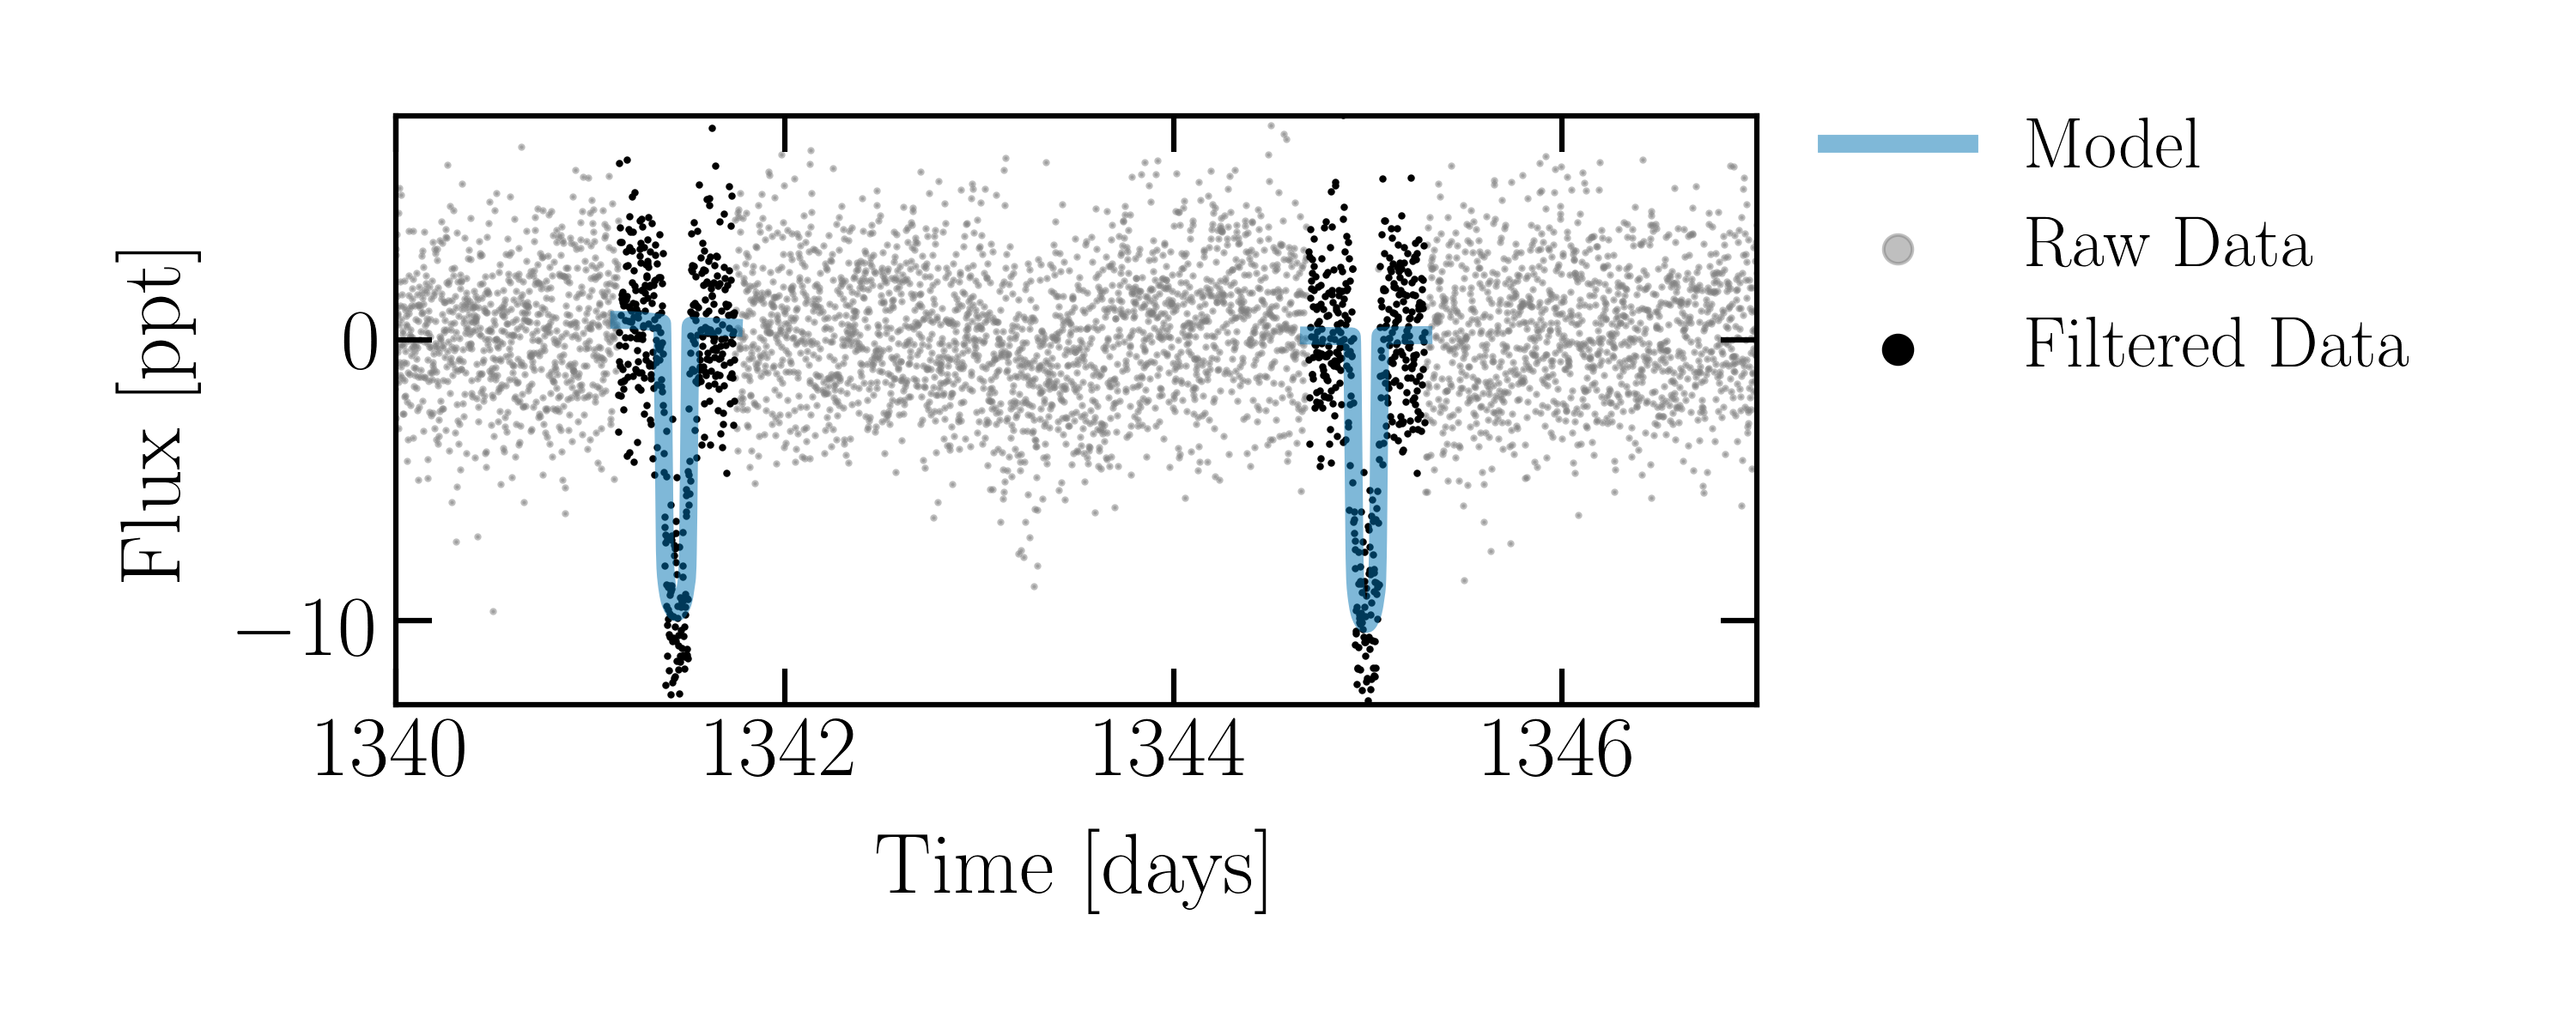
\includegraphics[width=\linewidth]{figures/raw_data_toi_103.png}
    \caption{\textbf{Light curve data for \TOI{103} (from 1030-1450 BKJD):} The raw light curve data for \TOI{103} is plotted in gray, with the \exofop\ transit model plotted on top in blue. The black points are obtained by filtering the raw data using the \exofop\ transit parameter estimates as described in the text. Code to reproduce this plot is on GitHub~\paperPlotsLink.}
    \label{fig:raw}
\end{figure*}

We obtain planetary parameters for \numTessCandidates TOIs with two-minute cadence data from the Exoplanet Follow-up Observing Program for TESS catalog~\citep[\exofop][]{Guerrero:2021:ApJS}.\footnote{Data was downloaded from \exofopLink\ on July 28, 2022.}
This catalog reflects the best possible analysis when promoting transit search candidates into TOIs~\citep{Guerrero:2021:ApJS}.
Any TOIs lacking a period measurement, or a period equal to zero, are flagged as single-transit systems.
We download the TOI light curves created by the TESS Science Processing Operations Center pipeline~\citep{Jenkins:2016:SPIE, Jenkins:2021:tsc2} using \lightkurve~\citep{LightkurveCollaboration:2018:ascl}.\footnote{All the \tess\ light curve data used in this paper can be found in \mast: \mastDatabase.}

As a preliminary step, the light curve is filtered to remove low-frequency outliers.
If the light curve dataset contains more than $100,000$ data points, an additional filtering step is performed: data outside the anticipated \exofop\ transit times (with a buffer of two times the expected transit duration) are discarded.
Figure~\ref{fig:raw} displays a plot of {TOI 103}'s raw and filtered light curves, as well as \exofop's transit model
Finally, parameter estimates for the radius and stellar density of each TOI's host star are retrieved from mast, if available.



\subsection{Transit Model}

The host star's limb darkening profile is approximated using \citet{Kipping:2013:MNRAS}'s quadratic limb darkening law \citep{Claret:2000:A&A, Mandel:2002:ApJL}, parameterised in \starry~\citep{Luger:2019:AJ} by the baseline relative flux of the light curve $f_0$ and two quadratic limb-darkening parameters $u_1, u_2$.
The stellar variability (from e.g. asteroseismic oscillation of the star) is modelled with a \celerite~\citep{Foreman-Mackey:2017:ascl} Gaussian Process (GP), with a stochastically driven damped harmonic oscillator kernel in linear combination with a jitter term $J$, to capture misspecified error bars and model misspecification.
The GP requires three parameters: the quality factor $Q_{\rm GP}$, the undamped period of the oscillator $\rho_{\rm GP}$, and the standard deviation of the process $\sigma_{\rm GP}$.
Exoplanet transits are modelled as circular (non-interacting) Keplerian orbits around their host star, using \exoplanet~\citep{Foreman-Mackey:2021:JOSS}.
Circular orbits permit the use of computationally efficient, analytical orbital dynamics calculations.
Additionally, circular orbits avoid degeneracies between eccentricity $e$, the argument of periastron $\omega$, impact parameter $b$, and planet radius $R_p$.
Furthermore, the eccentricity can also be computed in post-processing, as described by \citet{Dawson:2012:ApJ}.
Each of the $n$ exoplanets in a system is parameterised by
\begin{enumerate}
  \item \emph{two reference transit times}, one near the beginning of the observations, $\tmin[n]$, and one near the end, $\tmax[n]$, both measured in \tess\ BJD,
  \item \emph{the number of periods}, $N_P[n]$, in the \tess\ observational baseline, between $\tmin$ and $\tmax$,
  \item \emph{the transit duration}, $\tau[n]$, measured in hours,
  \item \emph{the orbital impact parameter}, $b[n]$, constrained to be $|b| \le 1$, and
    \item \emph{the radius ratio} $R_{\rm p}[n] / R_\star$, of the planet radius $R_{\rm p}[n]$ divided by the stellar radius $R_\star$.
\end{enumerate}
The radius ratio is computed from the approximate transit depth, $\delta[n]$, measured in parts-per-thousand, using the small planet approximation
\begin{equation}
    R_{\rm p}[n]/R_{\star} = \sqrt{\delta[n]}\, .
\end{equation}
Additionally, the orbital period, $P[n]$, measured in days, can be calculated for each planet as
\begin{equation}
  P[n] =  (\tmax[n] - \tmin[n]) / N_P[n]\, .
\end{equation}
If a planet only transits once in observed data ($N_P[n]=1$), we parameterize the model with $\{\tmin[n], P[n]\}$ instead of $\{ \tmin[n], \tmax[n]\}$.

\subsection{Inference Framework}

\textit{Noise and stellar parameter priors:}
Uninformative priors are set for the stellar limb darkening (using the \citet{Kipping:2013:MNRAS} parameterisation), mean flux, and noise parameters.
The quality factor $Q_{\rm GP}$ prior is fixed to a delta function at zero point three.

\textit{Transiting exoplanet priors:}
The transiting exoplanet parameter priors are centred around \exofop\ estimates.
As transiting planet’s phase and period are tightly constrained, we enforce a delta prior on the number of periods $N_P[n]$ between the two references times $\tmin[n]$ and $\tmax[n]$.
The reference time priors are centred near the anticipated transit times and allowed a wide range of up to ten times the \exofop\ transit duration.
If a planet only has a single-transit data recorded for a duration of time $t$, the prior on the second reference time $\tmax[n]$ is substituted with a prior on the planet's orbital period $P[n]$.
As the orbital period for a single-transit planet is challenging to measure, a wide Pareto prior is placed on the period, with the minimum period $P_{\rm min}$ equal to
\begin{equation}
P_{\rm min}[n] = \rm{max} \left\{ \begin{array}{cl}
\tmin[n] - {\rm min}(t)\\
{\rm max}(t) - \tmin[n]
\end{array} \right. \, .
\end{equation}
This prior provides more support for shorter periods.
Importantly note that  does not change the prior on $\tmin$ and $\tmax$ since the Jacobian is a constant $1/N_P$

We set a log-normal radius ratio prior, centred at the \exofop\ radius ratio measurement.
This radius ratio prior provides more support for systems with smaller ratios.
Finally, the impact parameter prior is uniform, conditioned on the radius ratio.
A full list of the priors is presented in Table~\ref{tab:priors}.

\begin{table*}[]
\centering
\caption{\textbf{Priors table:} Table of priors on the light curve transit model parameters. We use shorthand to represent distributions: $\Un$~uniform (min, max), $\N$~normal ($\mu,\sigma$), $\Par$~Pareto ($\alpha$, min) and finally $\invG$~Inverse Gamma (lower, upper). The prime superscript (${}^{\prime}$) indicates values from \exofop.  Each planet in a $n$-planet system will have its unique planet priors. The $t_i$ parameter is shorthand for both $\tmin$ and $\tmax$. The $P$ prior is used only for planets with a single transit in data in place of $\tmax$. $P_{\rm min}$ is defined in the text. Finally, the prior on $b$ is conditional on $R_{\rm p}/R_{\star}$ (refer to \exoplanet\ documentation for details.)}\label{tab:priors}
\def\arraystretch{1.1} 
\setlength{\tabcolsep}{0.5em}
\begin{tabular}{cllcl}
\text{Parameter}      & \text{Distribution}  &  & \text{Parameter}    & \text{Distribution}                                                    \\ 
\cline{1-2} \cline{4-5} 
\text{Star}           &                      &  & \text{Planet[$n$]}  &                                                                        \\
$u_1, u_2$            & $\Un(0,1)$           &  & $R_{\rm p}/R_\star$ & $\ln \N(R_{\rm p}^{\prime}/R_\star, 1)$                                \\
$f_0$                 & $\N(0, 10)$          &  & $b$                 & $\Un(0, R_{\rm p}/R_\star +1)$                                         \\                            
\text{Noise}          &                      &  & $\tau/\rm{days}$    & $\ln\N(\ln\tau^{\prime}, 0.2) \in [4\, \rm{min},  10\tau^{\prime}]$    \\
$\rho_{\rm GP}$       & $\invG(0.5, 10)$     &  & $t_i/\rm{TBJD}$     & $\N(t_i^{\prime}, \tau^{\prime}) \in [t_i^{\prime}\pm10\tau^{\prime}]$ \\
$ \sigma_{\rm GP}, J$ & $\invG(1, 5)$        &  & $P/\rm{days}$       & $\Par(2/3, P_{\rm min})$                                               \\
$ Q_{\rm GP}$         & 0.3                  &  & $N_P$               & $N^{\prime}_P$                                       
\end{tabular}    
\end{table*}


\textit{Posterior sampling:}
We initialise the posterior sampler at a high likelihood point, obtained by using \exoplanet's non-linear optimisation framework.
Following initial optimisation, the posterior distribution is sampled with \pymc's Hamiltonian Monte Carlo (HMC) No U-Turn Sampler~\citep{Hoffman:2011:arXiv,Betancourt:2017:arXiv,Salvatier:2016:ascl}.
The sampler is run on two chains for 4,000 steps with a burn-in of 2,000 steps.
We pass the chains to \arviz\ and compute the rank normalised $\hat{R}$ diagnostic statistic~\citep{Vehtari:2019:arXiv}.
Analyses with $\hat{R}>1.01$ are considered failures due to convergence issues.


\subsection{Eccentricity post processing}

For successful analyses, we conduct a post-processing step to compute the orbital eccentricity, $e[n]$, and argument of periapsis, $\omega[n]$, for each transiting planet.
We use our measurements of transit observables to compute the implied stellar density (under the assumption of circular orbits), $\rho_{\rm circ}[n]$.
The expression for $\rho_{\rm circ}[n]$ is derived in Appendix~\ref{apdx:stellar_density}.
Note that $\rho_{\rm circ}[n]$ is not the same as the actual stellar density, $\rho_{\star}$, and is unique for each planet in an $n$-planet system \citep[see, for example,][]{Dawson:2012:ApJ, Kipping:2012:MNRAS}.
Following \citet{Dawson:2012:ApJ}, we use $\rho_{\rm circ}[n]$ with a cataloged value of $\rho_\star$ (obtained from \mast) to generate weights.
These are used to re-weight uniformly drawn $e[n]$ and $\omega[n]$ to get weighted posterior samples.

\subsection{Execution and catalog generation}

From data retrieval to post-processing, the analysis steps for a TOI are implemented in a `template' \jupyter\ notebook.\footnote{\toiTemplateLink}
After duplicating the template for each TOI, we insert the TOI number into each notebook and execute them in parallel with \nbconvert.
After execution, we use \jupyterbook, a \sphinx-based package~\citep{sphinx_doc}, to convert the notebooks into web pages.
In addition to the analysis code, the pages display plots of the raw \mast\ and filtered light curves, HMC chain trace plots, posterior plots and phase-folded light curve plots of inferred orbits.
The pages are deployed to the \tessAtlas\ website, alongside the \jupyter\ notebooks, raw data (the light curve data and \exofop\ estimates) and analysis outputs (the HMC chains and re-weighted posteriors).
Finally, the median value and 1-$\sigma$ bounds of all TOI posterior distributions are reported.

\section{Results}\label{sec:results}


\subsection{Summary of the \tessAtlas\ catalog}

We analysed \numAnalysed\ two-minute cadence TOIs.
From these, \failPercent\ analyses failed, most of which were TOIs with grazing transits ($b\gtrsim0.9$).
The successful analyses include \numAnalysedSingle\ TOIs with a single transit in data and \numAnalysedMulti\ TOIs in systems with multiple planets (in a total of \numMultiSystems\ multi-planet systems).
The catalog website displays the results for each TOI.

\begin{figure}
  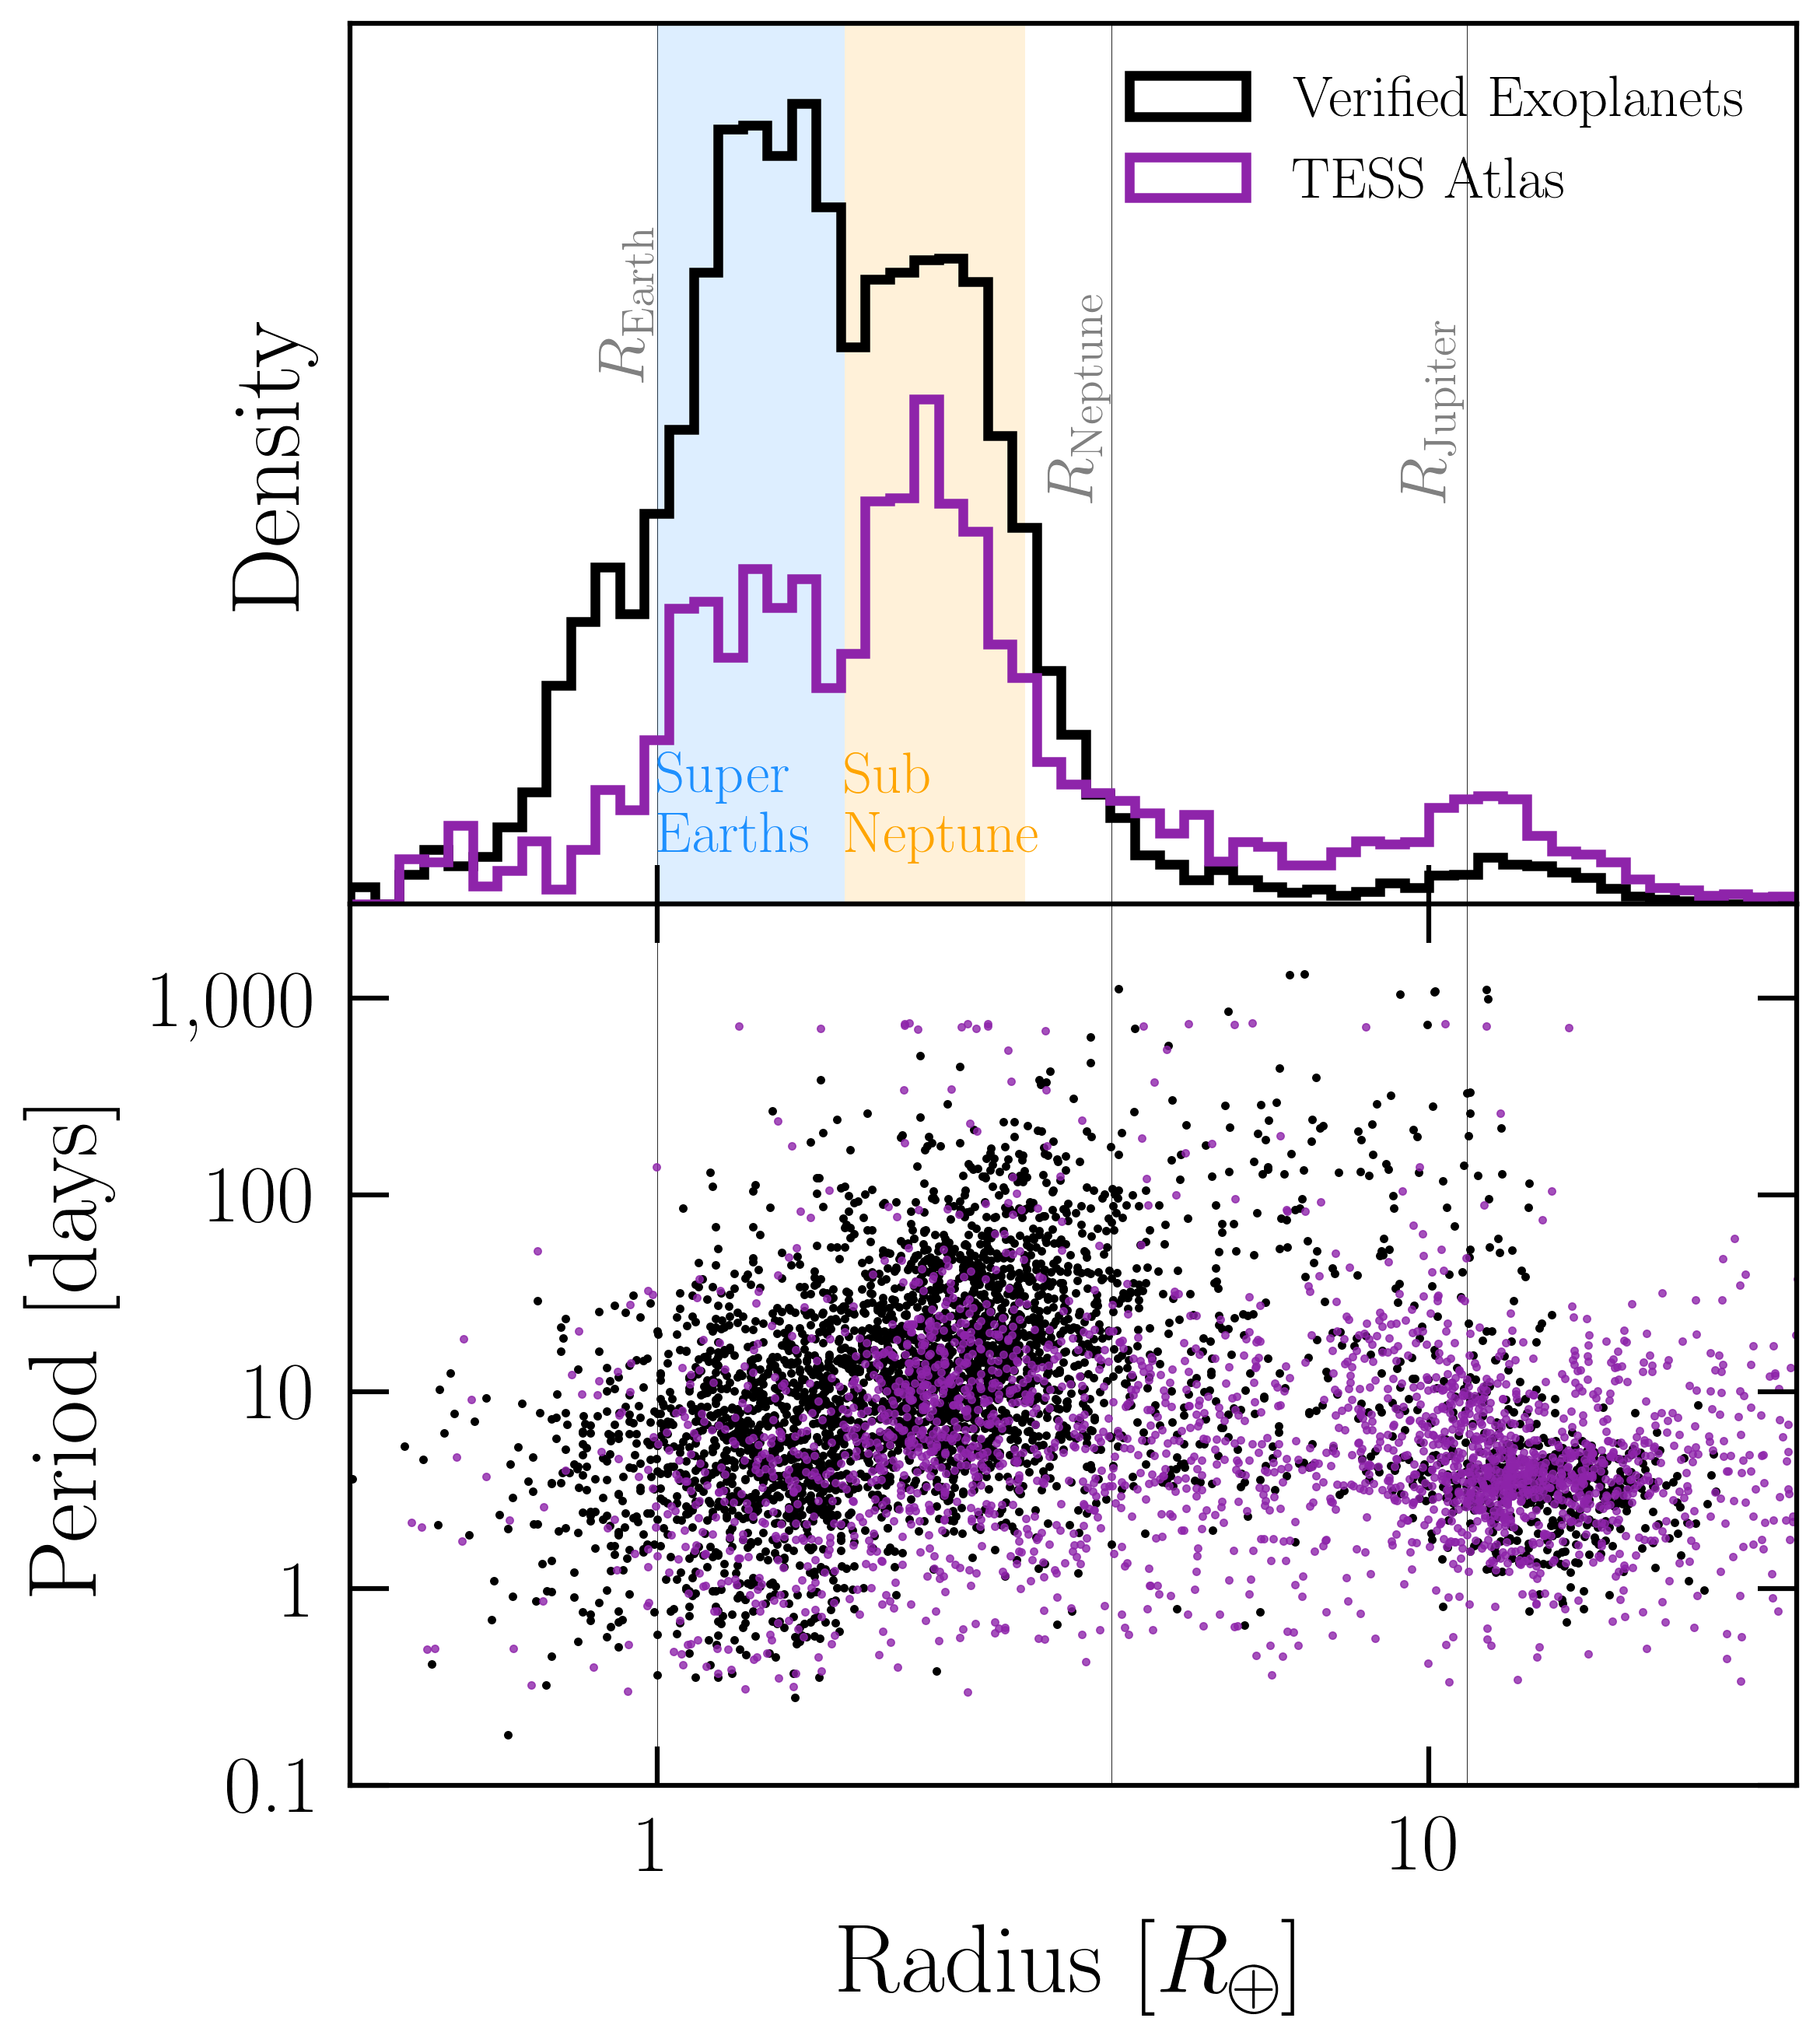
\includegraphics[width=\linewidth]{figures/radius_period_plot.png}
  \caption{\textbf{TOIs in period-radius space:}
    (Top) Planet radii distribution. (Bottom) Planet period vs. radius scatter plot.
    The purple data are from the \tessAtlas\ fits, while the black data are from the population of verified transiting exoplanets, obtained from NASA's exoplanet archive.
    The code to reproduce this plot is on GitHub~\paperPlotsLink.
  }
  \label{fig:radiusHist}
\end{figure}


Figure~\ref{fig:radiusHist} shows a plot of the \tessAtlas\ planetary periods and radii estimates (in purple).
The top of the Figure displays the planetary radii distribution.
We include the verified transiting exoplanet distribution from the NASA exoplanet archive (in black) to compare to the \tessAtlas\ catalog.\footnote{The NASA Exoplanet Science Institute's Planetary Systems Composite Table can be downloaded from \confirmedPlanetsDb.}
The \citet{Fulton:2017:AJ} radius-gap is visible in the minor depletion of planets with radii between super-Earths and sub-Neptunes in both catalog radii distributions.
Although the \tessAtlas\ has a lower super-Earth distribution, there is some agreement with the population of known exoplanets.


\subsection{Comparing with \exofop\ estimates}

\begin{figure}\label{fig:phase}
    \centering
    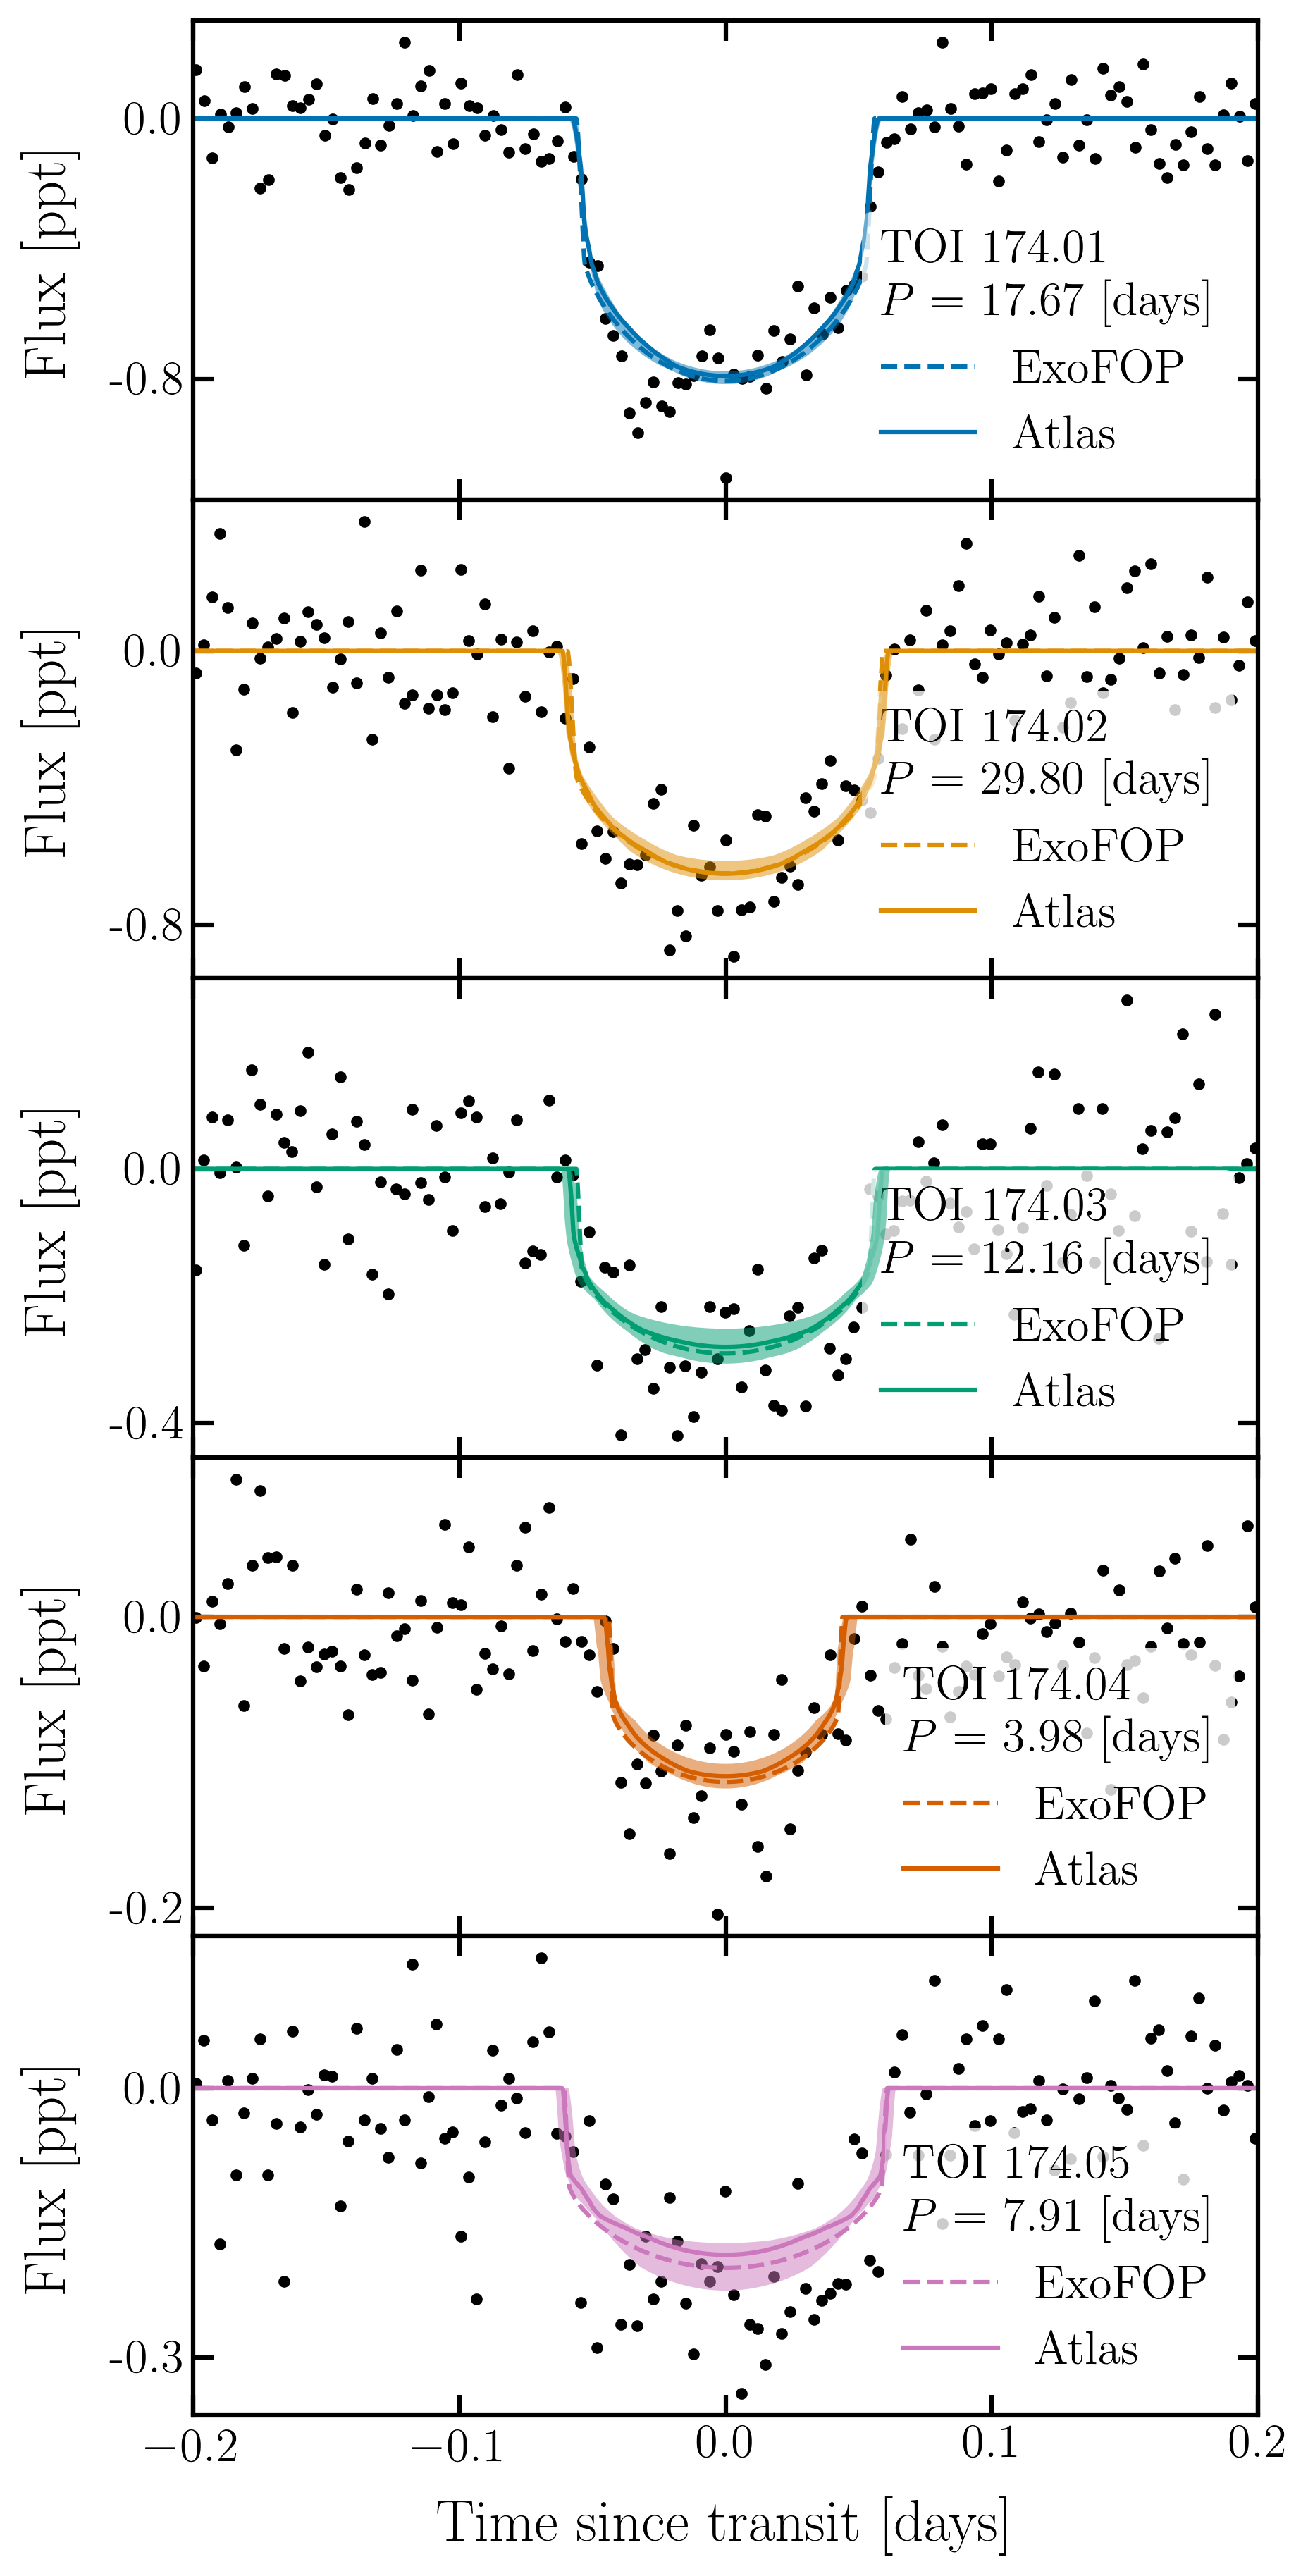
\includegraphics[width=0.9\linewidth]{paper/figures/toi_174_phase.png}
    \caption{\textbf{\TOI{174} phase-folded light curve plots:}
    De-trended light curves of the five \TOI{174.01-.05} planets, folded each at each TOI's period posterior median value.
    The light curve data points (black) are binned to reduce visual clutter.
    The shaded regions display the inferred orbits' posterior constraints (the 90\% CI region), while the solid curves show orbits from the posterior median value.
    Finally, the dashed curve depicts the model's orbits using \exofop\ orbital parameters.
    }
\end{figure}

\begin{figure*}\label{fig:posteriors}
    \centering
    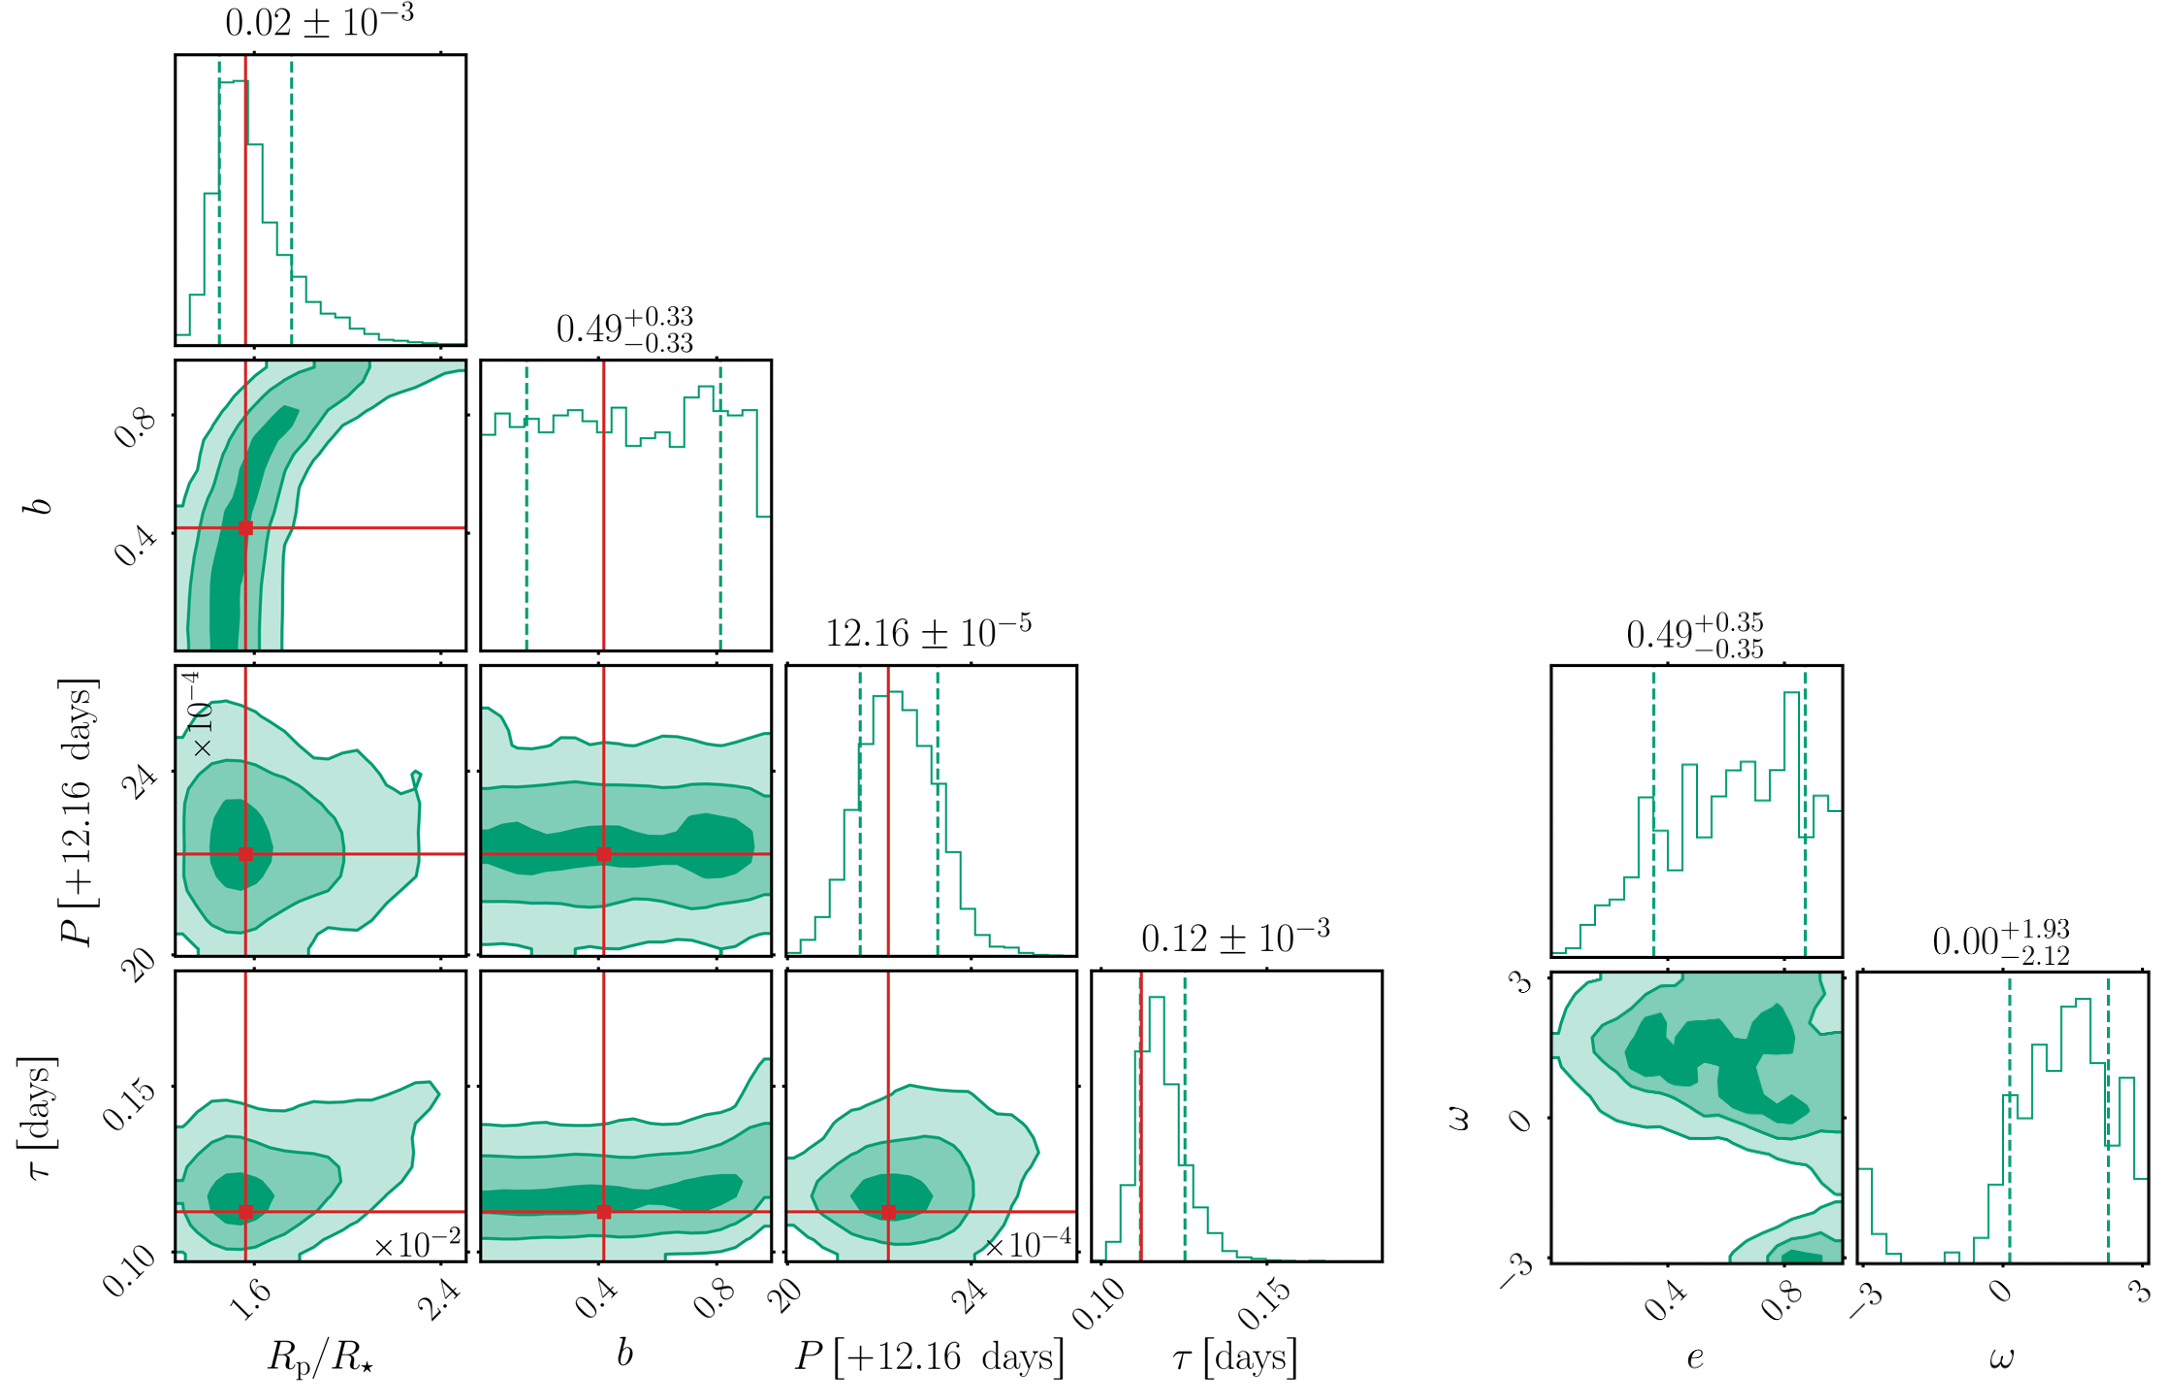
\includegraphics[width=0.9\linewidth]{figures/combined_posterior.png}
    \caption{\textbf{TOI 174.03 Posteriors:} (Left) Radius ratio $R_{\rm p}/R_\star$, impact parameter $b$, orbital period $P$ and transit duration $\tau$ posteriors. (Right) Re-weighted posteriors for eccentricity $e$ and the argument of periastron $\omega$.
    The shaded regions depict the 1,2,3-$\sigma$ contours. The 1D histograms dashed lines are the 90\% credible intervals (CI).
    The numbers above the 1D histograms are the posterior median values with the 90\% CI values as the uncertainties.
    The over-plotted red line indicates the \exofop\ transit parameters, except for $e$ and $\omega$.
    No values for $e$ and $\omega$ are provided on {TOI 174.03}'s \exofop\ page.
    Source code for this plot is provided in GitHub~\paperPlotsLink.}
\end{figure*}


To qualitatively assess the similarity between Atlas and \exofop\ inferred parameters, we superimpose \exofop\ measured values over the Atlas posterior and phase-folded light curve model plots.
Figure~\ref{fig:phase} shows the phase-folded light curve plots for all five planets in \TOI{174}.\footnote{The \tessAtlas\ catalog page for \TOI{174} can be found here: \toiPage{174}.}
Each row displays the model predictions for one of the five planets.
The datasets are folded on each planet's median period posterior value.
The model's inferred orbits and 90\% credible interval (CI) range are also folded and plotted in color on top of the black light curve data points.
The model predictions using the \exofop\ orbit parameters are displayed with the dashed curves.
The \exofop\ transit orbit parameters fall within the Atlas' 90\% CI range, demonstrating visual consistency.
This consistency between parameter estimates is highlighted in \TOI{174.03}'s posterior plot in Figure~\ref{fig:posteriors}.
The \exofop\ $R_{\rm p}/R_{\star}, b, P, \tau$ values are plotted in red over the posteriors and lie within the 1-$\sigma$ regions.


\begin{figure}\label{fig:frac_diff}
  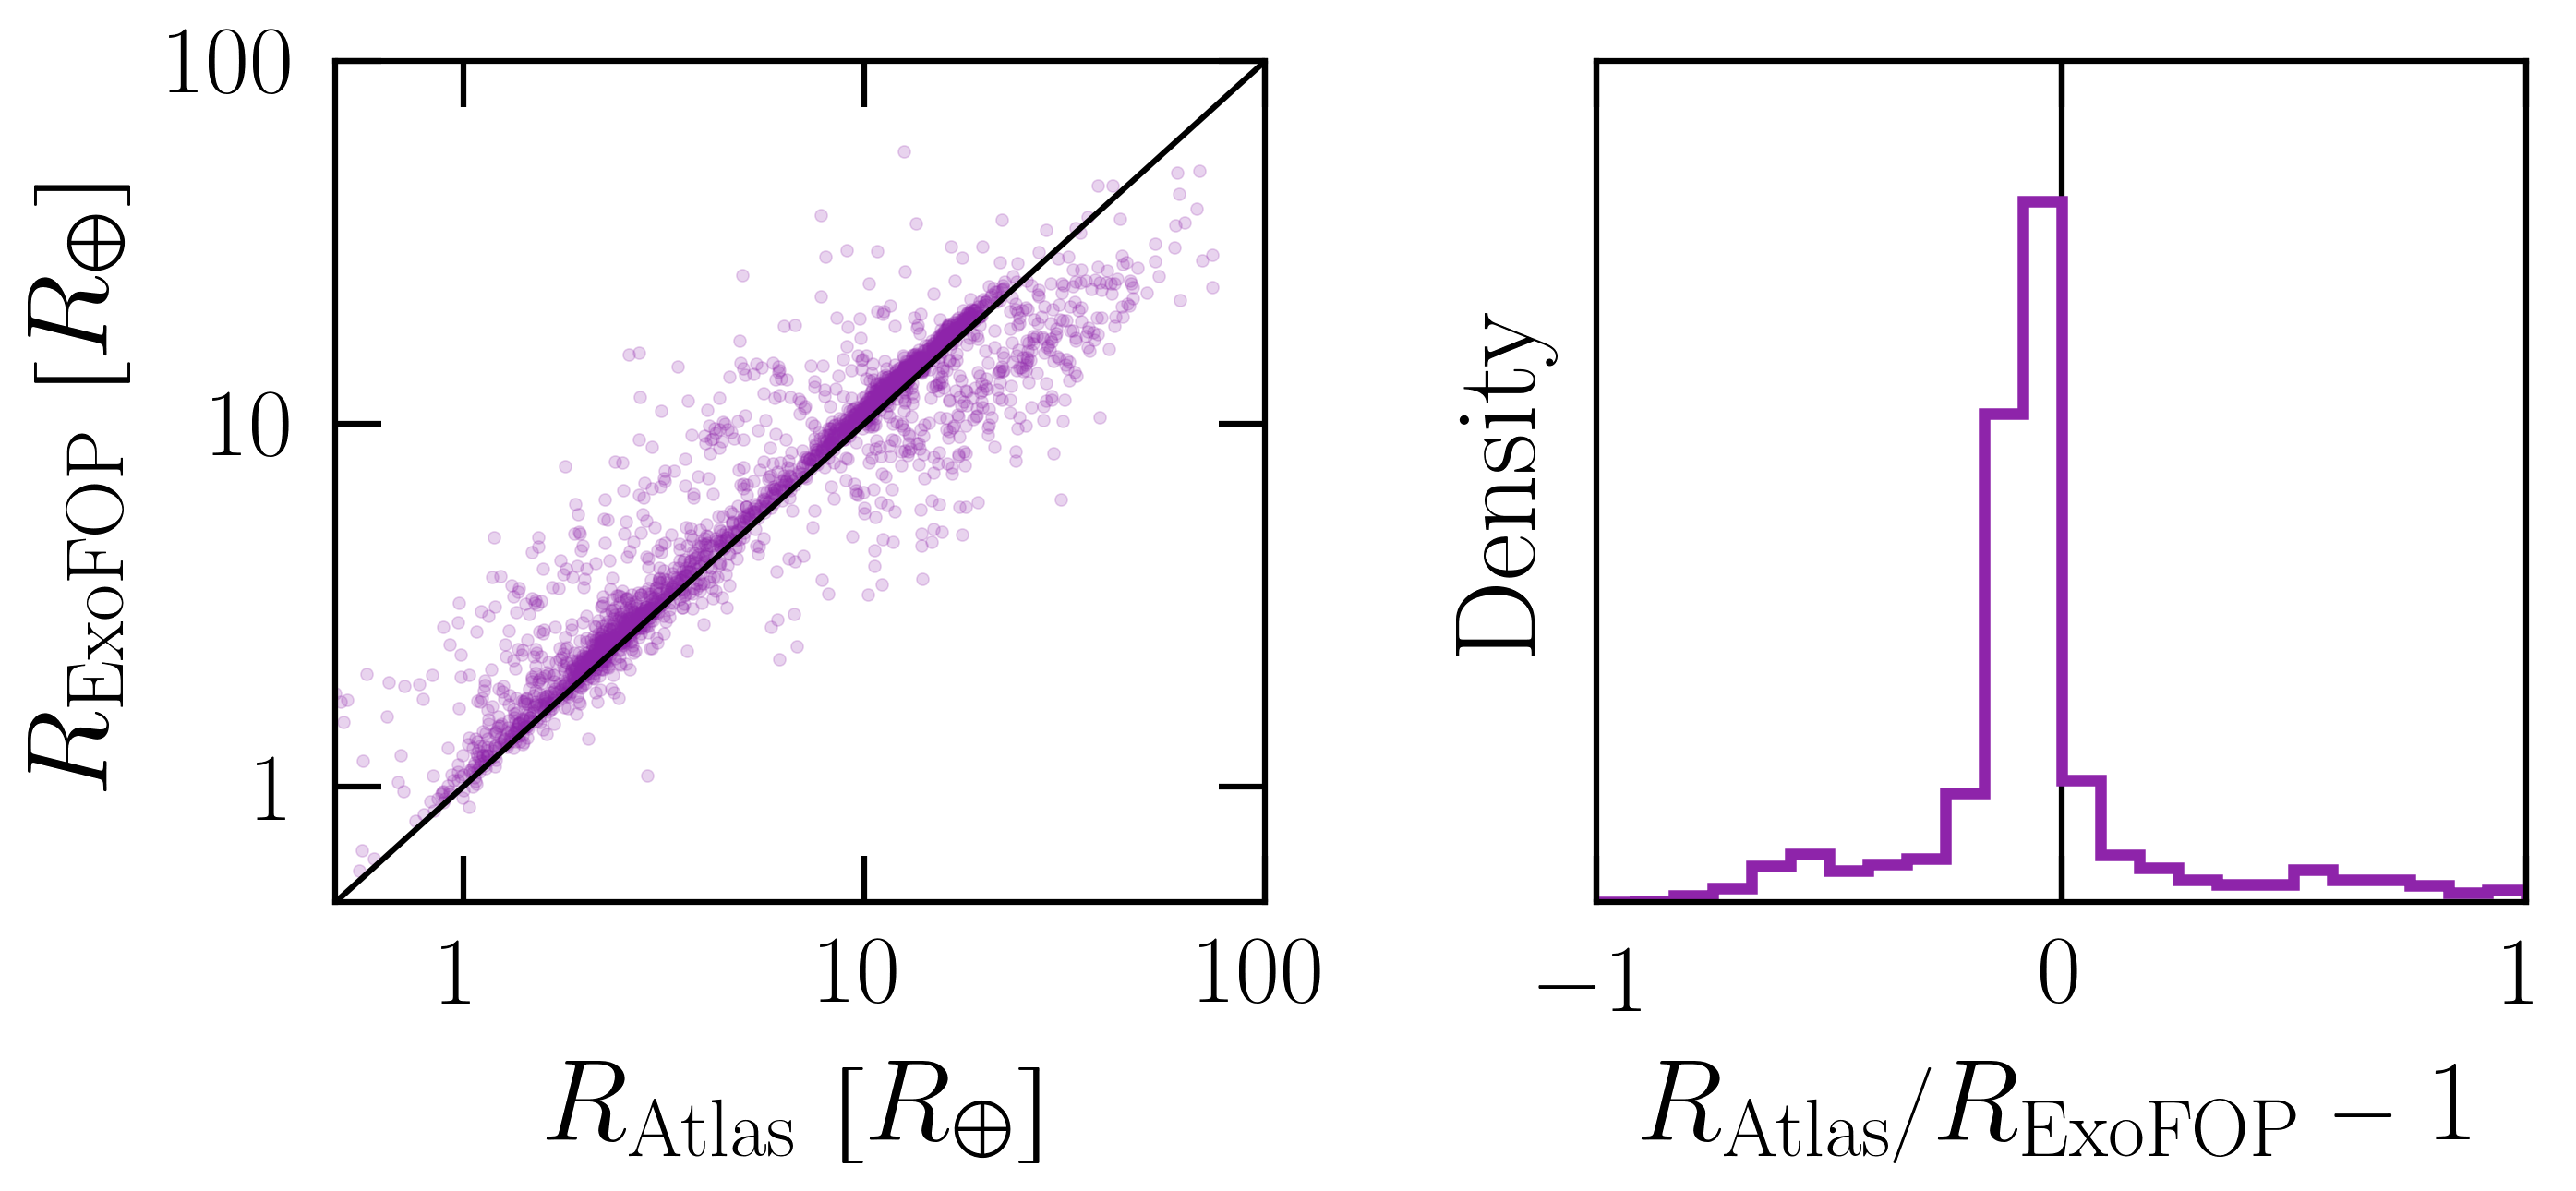
\includegraphics[width=\linewidth]{figures/radius_error.png}
  \caption{\textbf{Comparison of \exofop\ and \tessAtlas\ radii measurements:} (Left) A scatter plot of the \exofop\ TOI radii, $R_{\rm ExoFOP}$, against the \tessAtlas\ TOI radii estimates, $R_{\rm Atlas}$.
  The black line shows the one-to-one correspondence.
  (Right) Distribution of fractional change in planet radii between the two catalogs.
  Source code for this plot is provided in GitHub~\paperPlotsLink.
  \avi{Try coloring the left data points by impact parameter -- i think the large impact parameter events are the ones with differing radii.}
  }
\end{figure}

We estimate each TOI's $R_{\rm p}$ by multiplying the \tessAtlas\  median $R_{\rm p}/R_{\star}$ posterior value with the \mast\ stellar radii.
To compare the \tessAtlas\  and \exofop\ catalog radii, we plot the two sets of radii against one another on the left side of Figure~\ref{fig:frac_diff}, while the right side displays the distribution of fractional change in planet radii between the two catalogs.
The black line plotted in both panels shows the 1:1 line between the two sets of posterior estimates.
The TOIs with similar parameter estimates in both catalogs are found along this line.
We find 80.3\% of TOIs have \tessAtlas\ and \exofop\ radii estimates within 1-$\sigma$ of each other.
The median value of the fractional change plotted on the right side of  Figure~\ref{fig:frac_diff} is -7.2\% with a standard deviation of 39.8\%, indicating that \tessAtlas\ radii are systematically smaller than those in \exofop.
Additionally, we find 3.7\% of TOIs have radii that differ between the catalogs by more than $3\sigma$.
These discrepancies are attributable to variations between the \tessAtlas\ and \exofop\ analyses, including the data detrending method  and the model parameterisation.
Some of these TOIs may have $b\gtrsim0.7$, in turn leading to inaccurate sampling~\citep[see e.g.][]{Thompson:2018:ApJS, Gilbert:2022:AJ}.
Calculating the fractional difference between the \exofop\ and \tessAtlas\ period measurements, excluding systems with only a single transit, we see that the two catalogs are very consistent ($\sim95\%$ of TOIs have a period fractional difference of less than $1\%$).


\section{Discussion and caveats}\label{sec:conclusion}
We present the first catalog of transiting exoplanet posterior distributions for TOIs with two-minute cadence data from 2018-2021.
All posterior files and software for this study are made available to the public via supplementary materials.
However, there are a few caveats to be aware of when using the catalog.
First, we model \textit{all} TOIs with a circular transit model, including those non-planet dispositions.
Additionally, the circular transit approximation substantially overestimates the constraints on the impact parameter constraint~\citep
{Gilbert:2022:AJ}. For better measurements of the impact parameter,\citet{Gilbert:2022:AJ}'s umbrella sampling method with a grazing and non-grazing model should be used.
Second, the orbits are modelled as non-interacting, even in the case of a multi-planet system. In multi-planet systems, gravitational interaction can alter planet orbits, resulting in transits that are unevenly spaced.
Thirdly, transit timing variations, correlated noise, and other systematics are disregarded.
Incorporating these can significantly improve parameter measurements~\cite{Coughlin:2016:ApJS, Thompson:2018:ApJS}.
Finally, no statistical tests other than the $\hat{R}$ check were performed to verify sampler convergence; hence, portions of the catalog may have unconverged posteriors.
However, even with these caveats, our transit analysis will be useful not only as a catalog for transiting exoplanet parameters but also as a starting point for future work on individual TOIs, with the supplementary \jupyter\ notebooks.
As longer-duration light curves are developed, and more TOIs are made available to the public, we will periodically update the \tessAtlas\ database.

\section{Data and software availability}\label{sec:data}
We obtain the list of candidates from \exofop's publicly-accessible TOI page~\citep{Akeson:2013:PASP}, and use publicly-available light curve data (\mast: \mastDatabase). We compare our results against the publicly-available Planetary Systems Composite Table created by the NASA Exoplanet Science Institute (\confirmedPlanetsDb). We make our software (\atlasGit) and results (\atlasUrl) publicly accessible online. We additionally provide an application programming interface (API) to ease access to our data. The API is documented in the GitHub repository for this work.



%%%%%%%%%%%%%%%%%%%%



\section*{Acknowledgments}{

This work began during the `online.tess.science' workshop in September 2020.
The authors thank David Liptai, the OzStar and Nectar Openstack helpdesks, and the \lightkurve\ developers for technical assistance. We also acknowledge discussions and historical contributions made by Nicholas Saunders, Joel Ong, Geert Barentsen and Jason Rowe.
\avi{Should we invite them on this paper?}

We gratefully acknowledge the Swinburne Supercomputing OzSTAR Facility for computational resources. All analyses (including test and failed analyses) performed for this study used $127.6$K core hours on OzSTAR. This would have amounted to a carbon footprint of ${\sim13{\text{t CO}_2}}$~\citep{greenhouse, energy_to_co2_converter}. Thankfully, as OzSTAR is powered by wind energy from Iberdrola Australia; the electricity for computations produces negligible carbon waste.

The catalog is hosted on the Nectar Research Cloud by Swinburne University of Technology. The Nectar Research Cloud is a collaborative Australian research platform supported by the NCRIS-funded Australian Research Data Commons (ARDC).

This work has used the TIC through the TESS Science Office’s target selection working group (architects K. Stassun, J. Pepper, N. De Lee, M. Paegert, R. Oelkers). This research has used the NASA Exoplanet Archive, which is operated by the California Institute of Technology, under contract with the National Aeronautics and Space Administration under the Exoplanet Exploration Program. Some of the data presented in this paper were obtained from the Mikulski Archive for Space Telescopes (MAST) at the Space Telescope Science Institute. The specific observations analyzed can be accessed via \mastDatabase. STScI is operated by the Association of Universities for Research in Astronomy, Inc., under NASA contract NAS5–26555. Support to MAST for these data is provided by the NASA Office of Space Science via grant NAG5–7584 and other grants and contracts.

A.V. is supported by the Australian Research Council (ARC) Centre of Excellence CE170100004.
\avi{Get dan's dets}
}

\vspace{5mm}
\facilities{\tess, \mast, Exoplanet Archive.}

\software{
\python~\citep{pythonForScientificComputing,pythonForScientists},
\astropy~\citep{astropy},
\arviz~\citep{arviz_2019},
\exoplanet~\citep{Foreman-Mackey:2021:JOSS},
\lightkurve~\citep{LightkurveCollaboration:2018:ascl},
\starry~\citep{Luger:2019:AJ},
\celerite~\citep{Foreman-Mackey:2017:ascl},
\pymc~\citep{Salvatier:2016:ascl},
\numpy~\citep{numpy},
\scipy~\citep{SciPy},
\pandas~\citep{pandas},
\matplotlib~\citep{matplotlib},
\corner~\citep{corner},
\sphinx~\citep{sphinx_doc},
\jupyter~\citep{jupyter},
\jupyterbook~\citep{jupyter_book}.
}


% ADS bibliography link
% https://ui.adsabs.harvard.edu/user/libraries/_DyLS4HbTY-eJIMBiFUdxw
\bibliography{atlas}{}
\bibliographystyle{aasjournal}

%%%%%%%%%%%%%%%%%%%%%%%%%%%%%%%%%%%%%%%%%%%%
\appendix

\section{Computing the implied stellar density}\label{apdx:stellar_density}
For a circular orbit, the transit duration is \citep{Winn:2010:arXiv}
\begin{equation}~\label{eq:tau}
  \tau = \frac{P}{\pi}\,\sin^{-1}\left( \frac{\sqrt{(1 + (R_{p}/R_{\star})^2) - b^2}}{a\,\sin i} \right) \quad. \,
\end{equation}
where $a$ is the semi-major axis in units of $R_\star$.
Rearranging Eq~\ref{eq:tau} in terms of $a$, we find that
\begin{equation}~\label{eq:a1}
  a^2\,\sin^2 i\,\sin^2\left(\frac{\pi\,\tau}{P}\right) = (1 + (R_{p}/R_{\star})^2) - b^2 \quad.
\end{equation}
Since $\cos^2 i = b^2 / a^2$, Eq~\ref{eq:a1} can be simplified
\begin{equation}
  a^2 = \frac{(1 + R_{p}/R_{\star})^2 - b^2\,\cos^2\phi}{\sin^2\phi}
\end{equation}
for $\phi = \pi\,\tau / P$.

Finally, under the assumption of a circular orbit, we can compute the implied stellar density $\rho_\mathrm{circ}$ with the period and semi-major axis
\begin{equation}
  \rho_\mathrm{circ} = \frac{3\,\pi\,a^3}{G\,P^2} \quad.
\end{equation}



\end{document}
